\documentclass[a4paper]{article}
\usepackage{fullpage} % Package to use full page
\usepackage{parskip} % Package to tweak paragraph skipping
\usepackage{tikz} % Package for drawing
\usepackage{amsmath}
\usepackage{hyperref}
\usepackage{amssymb}
\usepackage{listings}
\usepackage{enumerate}
%%%%%%
\usepackage{graphicx}
\usepackage{pdflscape}
\usepackage{subfigure}
\usepackage{caption}
\captionsetup{aboveskip=0pt}
\usepackage{color}

\definecolor{mygreen}{rgb}{0,0.6,0}
\definecolor{mygray}{rgb}{0.5,0.5,0.5}
\definecolor{mymauve}{rgb}{0.58,0,0.82}

\lstset{ %
  backgroundcolor=\color{white},   % choose the background color; you must add \usepackage{color} or \usepackage{xcolor}; should come as last argument
  basicstyle=\footnotesize,        % the size of the fonts that are used for the code
  breakatwhitespace=false,         % sets if automatic breaks should only happen at whitespace
  breaklines=true,                 % sets automatic line breaking
  captionpos=b,                    % sets the caption-position to bottom
  commentstyle=\color{mygreen},    % comment style
  deletekeywords={...},            % if you want to delete keywords from the given language
  escapeinside={\%*}{*)},          % if you want to add LaTeX within your code
  extendedchars=true,              % lets you use non-ASCII characters; for 8-bits encodings only, does not work with UTF-8
  frame=single,                    % adds a frame around the code
  keepspaces=true,                 % keeps spaces in text, useful for keeping indentation of code (possibly needs columns=flexible)
  keywordstyle=\color{blue},       % keyword style
  language=Octave,                 % the language of the code
  morekeywords={*,...},           % if you want to add more keywords to the set
  numbers=left,                    % where to put the line-numbers; possible values are (none, left, right)
  numbersep=5pt,                   % how far the line-numbers are from the code
  numberstyle=\tiny\color{mygray}, % the style that is used for the line-numbers
  rulecolor=\color{black},         % if not set, the frame-color may be changed on line-breaks within not-black text (e.g. comments (green here))
  showspaces=false,                % show spaces everywhere adding particular underscores; it overrides 'showstringspaces'
  showstringspaces=false,          % underline spaces within strings only
  showtabs=false,                  % show tabs within strings adding particular underscores
  stepnumber=2,                    % the step between two line-numbers. If it's 1, each line will be numbered
  stringstyle=\color{mymauve},     % string literal style
  tabsize=2,                       % sets default tabsize to 2 spaces
  title=\lstname                   % show the filename of files included with \lstinputlisting; also try caption instead of title
}


%%%%%%
\title{Assignment 1 for \#70240413 \\ "Statistical Machine Learning" }
\author{Kui XU, 2016311209}
\date{2017/06/02}

\begin{document}

\maketitle

\section{Preparation}

\textbf{Summary}: 
\begin{enumerate}
\item[(1)] Python is my basic programming language, I use it everyday.
\item[(2)] And numpy is a very famous python package and I can not programming without it yet. 
\item[(3)] For Tensorflow, I am still a junior user, so I learn more in doing this homework.
\item[(4)] For ZhuSuan, a very great bayesian network library, a new programming mode for us to design a bayesian network by our self. I am a new user, I read a lot of documents to understanding the concepts of ZhuSuan, and I try to learn the programming mode by following the tutorial of VAE.
\end{enumerate}


\section{Variational inference for 2-D Gaussian Mixture}

\subsection{Write the variational lower bound}
In a simplest way, the variational lower bound $L(\theta, \Phi, x)$ is:
\begin{equation}
    \begin{aligned}
        L(\theta, \Phi, x) &= E_{q(z|x;\Phi)}[\log p(z,x;\theta) ] - KL(q z|x;\Phi) ‖ p(z; \theta))\\
    \end{aligned}
\end{equation}

$KL(q z|x;\Phi) ‖ p(z; \theta)) \le 0 $ depends on how goods $q(z|x)$ can approximate $p(z|x)$, so 
$E_{q(z|x;\Phi)}[\log p(z,x;\theta) ]$ is the lower variational bound of the (log) likelihood,  
$KL(q z|x;\Phi) ‖ p(z; \theta)) = 0 $ for perfect approximation.
\\
For $X$ is a Gaussian distribution, the lower bound is :

\begin{equation}
    \begin{aligned}
        E_{q(z|x;\Phi)}[\log p(z,x;\theta)]  &= - \log p(x|z)\\
        & = \sum \frac{1}{2} \log{\sigma_Z^2} +  \frac{(x-\mu_Z)^2}{2\sigma_Z^2} \\
        Z &\sim Discrete(\pi)
 \end{aligned}
\end{equation} 

Because of $Z \sim Discrete(\pi)$ is a Discrete distribution, which zs.sgvb only works for continuous latent  `StochasticTensor` s that can be reparameterized, we can not use zs.sgvb to 
estimate the gradient, we could use the zs.nvil function which can do the estimation both on continuous and discrete latent  `StochasticTensor`.

\subsection{Detailed Description}
Here, firstly I introduce the model (named GVAE model). Based on the 
pre-designed model,  it uses $Discrete(\pi)$ as the prior for $Z$; and uses 
$N(\mu_{Z^{i}}, diag\{\sigma_{Z^{i}}^{2}\})$ as the prior for $X$.
\\


In this model , the variational posterior distribution is 
\begin{equation}
    \begin{aligned}
        q(z,x;\Phi) &=  N(\mu_{Z}, diag\{\sigma_Z^2\})\\
        Z &\sim Discrete(\pi)
    \end{aligned}
\end{equation} 
 $q(z|x)$ is Gaussian distribution, and the variational parameter $z$ is a Discrete distribution, it would be the $\pi$ of the latent variables for each data point $\lambda_{x_i} = (\pi_{x_i})$, 
Here I design a feed forword neural network to learn the best $\pi$, the network consist of two layer fully connected, and I also try to increase the number of the layer, results is showed blew.
 How can we know how well our variational posterior $q(z|x)$ approximates the true posterior $p(z|x)$? We can use the Kullback-Leibler divergence.



\subsection{Data set}
The dataset is sampled with three fixed point, with $\mu \in (-0.2, 0.2, 0.6)$, $\sigma \in (0.1, 0.1, 0.1)$, for each pair of $\mu , \sigma$, I sampled 100 points, totally 300 point in to trainning set. The three big red points are the initial cluster center in an experiment. Figure 1 shows the data distribution.

\begin{figure}[!htbp]
\begin{center}
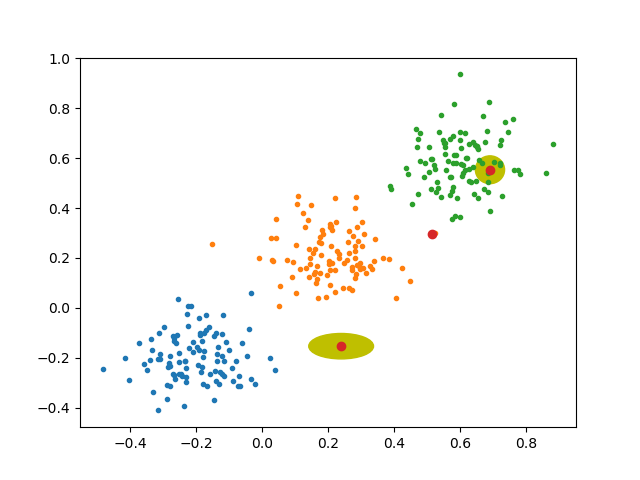
\includegraphics[width=14cm]{imgs/100_learn.png}
\end{center}
\caption{The figure shows the sampled data by three fixed point.}\label{datavis}
\end{figure}


\subsection{Experiment Setting}

\begin{enumerate}
\item[(1)] AdamOptimizer with Learning rate: 0.0001.
\item[(2)] Using $zs.nvil$ to estimate the gradient.
\item[(3)] Minimize the surrogate cost instead of lower bound.

\end{enumerate}

\textbf{Importance of initialization}:\\
In the code, in order to initialize a better $\pi, \mu, \sigma$, I initialize $\pi$ by using $`tf.constant\_initializer`$ with np.random.dirichlet(np.ones(K),size=1) for which a random dirichilet distribution can generate a vector with sum equal to 1; for $\mu$ and $\sigma$, I initialize them by using $`tf.random\_uniform\_initializer`$ with the range of val based on the data.
\\\\
Running on Tensorflow 1.1.0, K80-GPU, Ubuntu 14.04.
\subsection{Results}

I visialized the movement of the cluster center points step by step, showed in Figure 2. We can see that the cluster centers move to the point clouds step by step.

\begin{figure}[!htbp]
\begin{center}
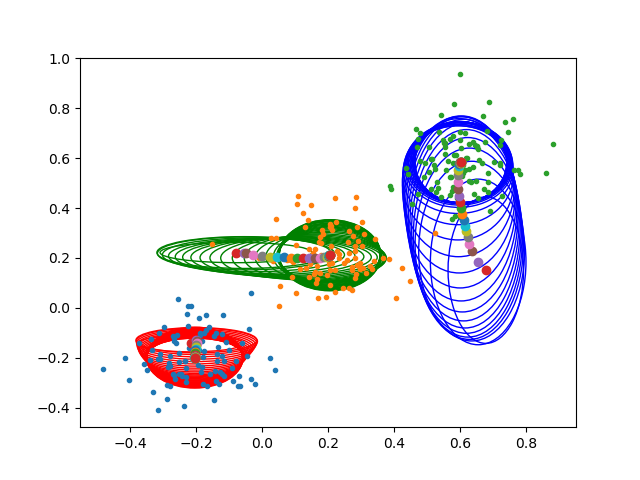
\includegraphics[width=16cm]{imgs/change_learn-2.png}
\end{center}
\caption{The movement of the cluster center via 3000 epochs}\label{changed}
\end{figure}


For a clear status of each epoch, I plot them and show them below:

\begin{landscape}
\begin{figure}
\centering
\subfigure[Epoch 10]{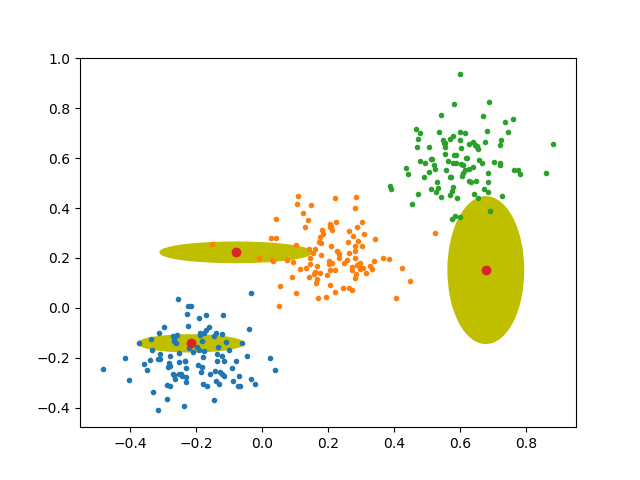
\includegraphics[width=6cm]{gmm2/10_learn.png}}
\subfigure[Epoch 100]{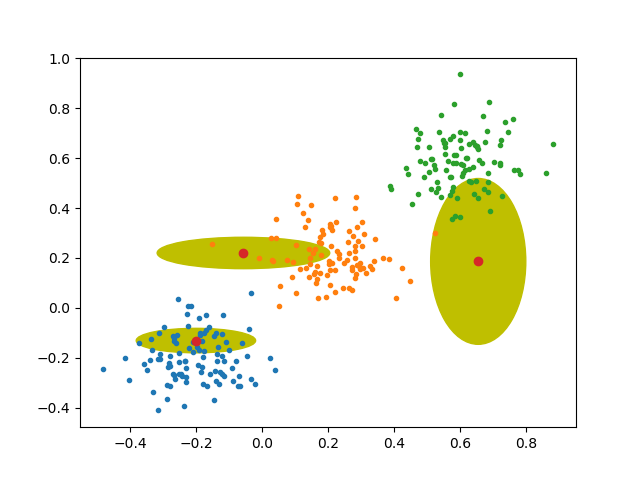
\includegraphics[width=6cm]{gmm2/100_learn.png}}
\subfigure[Epoch 500]{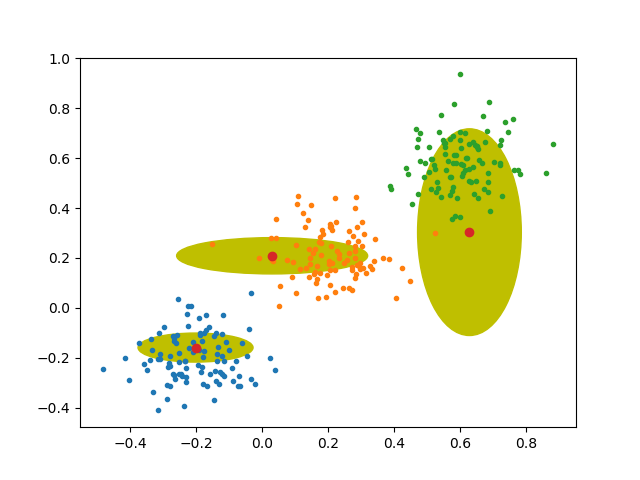
\includegraphics[width=6cm]{gmm2/500_learn.png}}
\vskip3ex
\subfigure[Epoch 800]{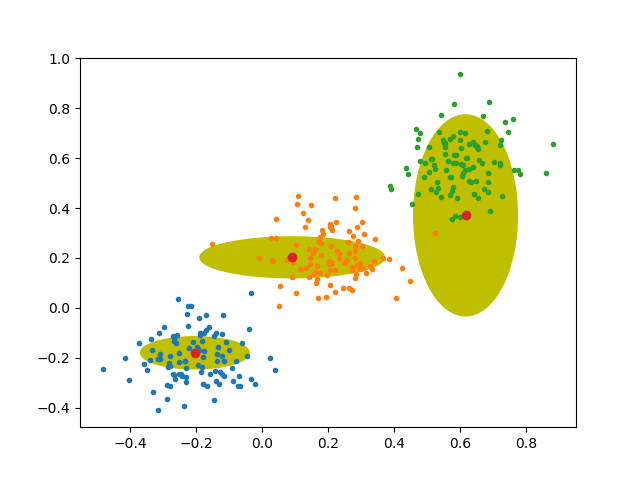
\includegraphics[width=6cm]{gmm2/800_learn.png}}
\subfigure[Epoch 1200]{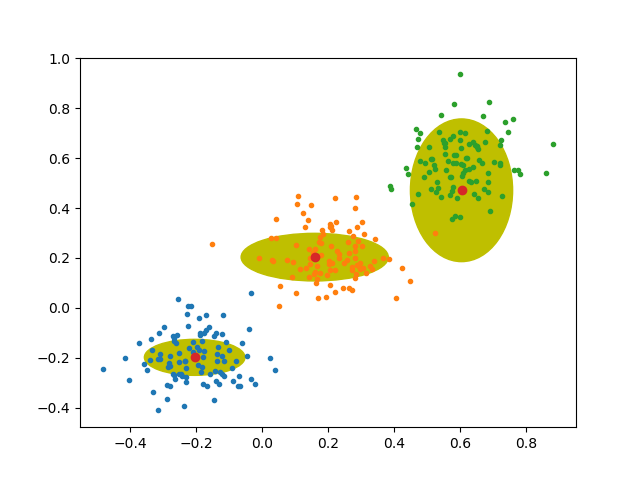
\includegraphics[width=6cm]{gmm2/1200_learn.png}}
\subfigure[Epoch 1800]{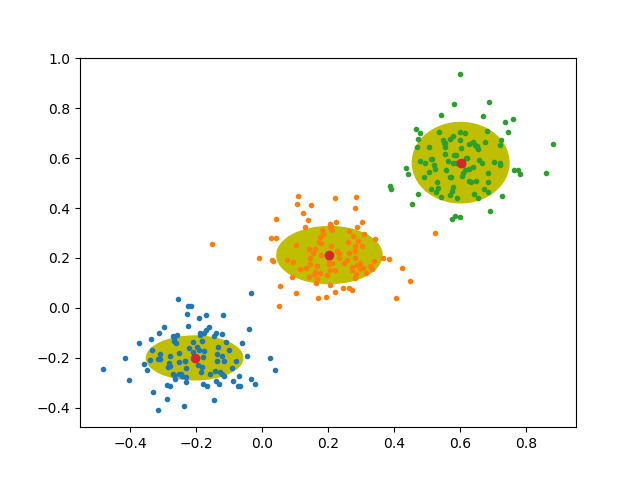
\includegraphics[width=6cm]{gmm2/1800_learn.png}}
\vskip3ex
\subfigure[Epoch 2000]{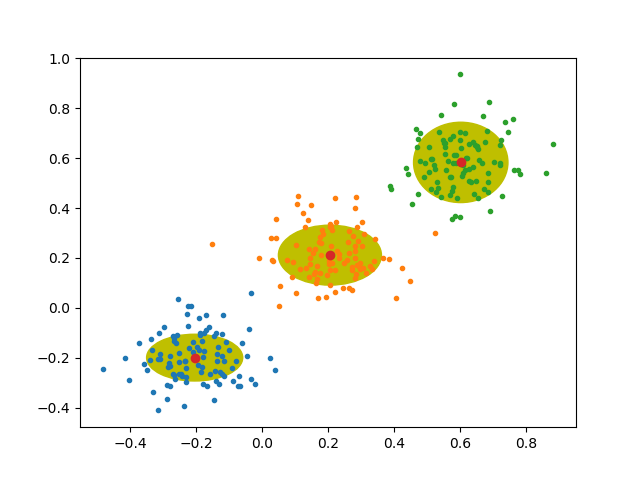
\includegraphics[width=6cm]{gmm2/2000_learn.png}}
\subfigure[Epoch 2500]{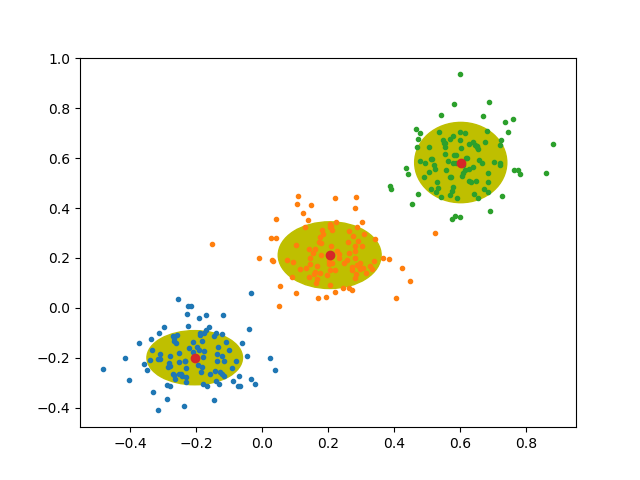
\includegraphics[width=6cm]{gmm2/2500_learn.png}}
\subfigure[Epoch 3000]{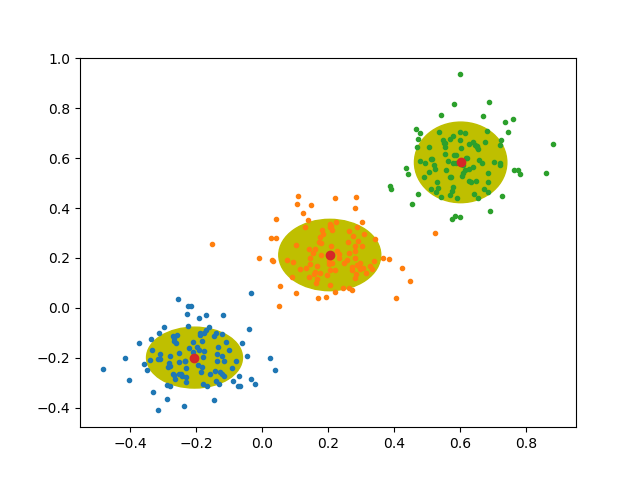
\includegraphics[width=6cm]{gmm2/3000_learn.png}}
\caption{Experiment 1: Two layer  The cluster center is changed over the epoch.}
\end{figure}
\end{landscape}

The surrogate cost shows that the training is convergent in 100 epoch. The low bound and the surrogate cost are near to zero.

\begin{figure}[!htbp]
\begin{center}
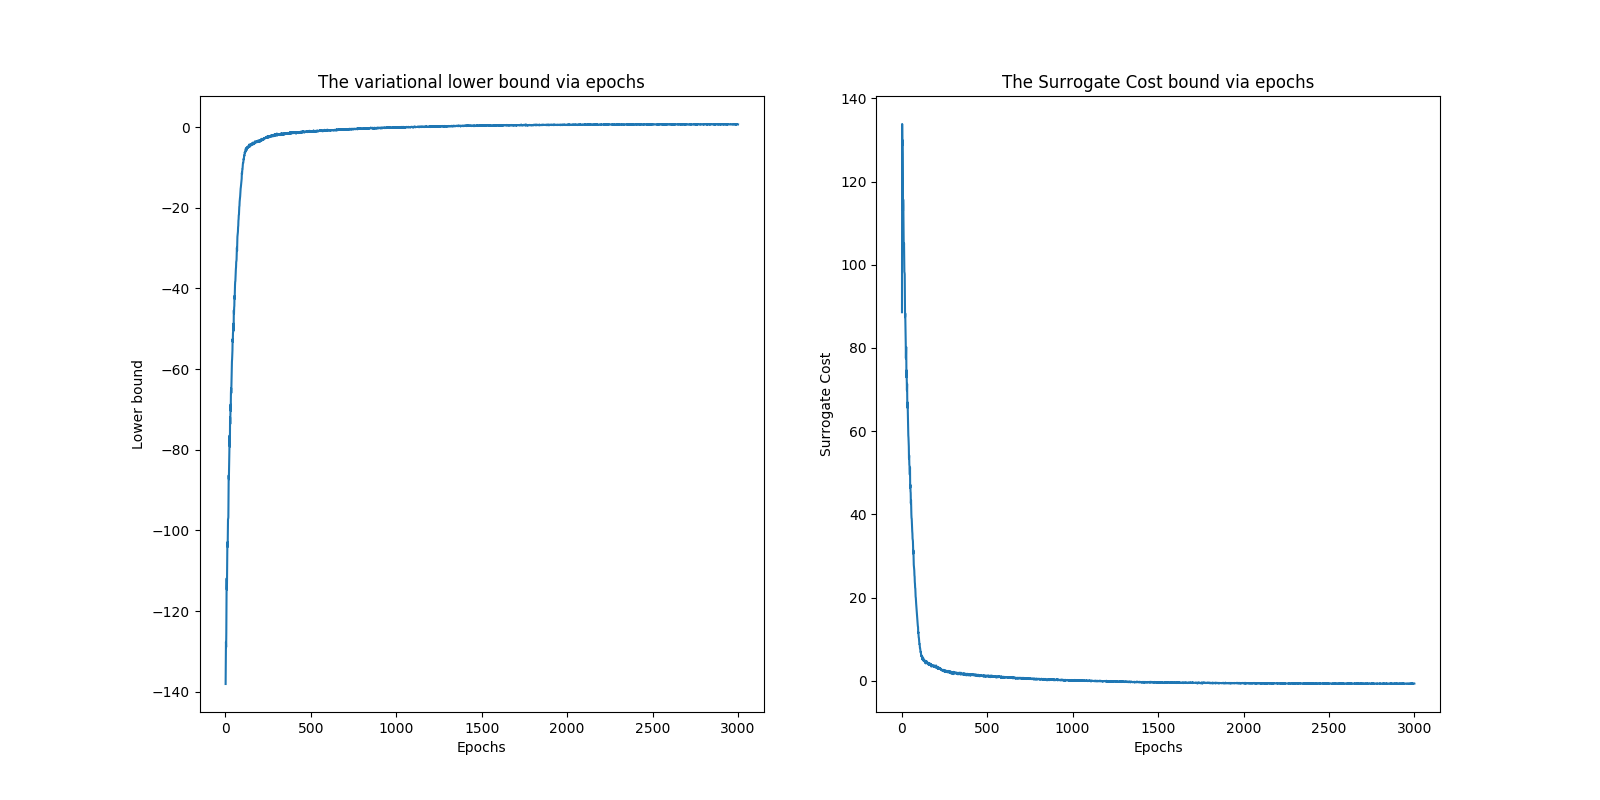
\includegraphics[width=18cm]{imgs/cost_lb.png}
\end{center}
\caption{The variational lower bound and surrogate cost via epochs.}\label{datavis}
\end{figure}


% \begin{sidewaysfigure}
% \subfigure[Epoch  A]{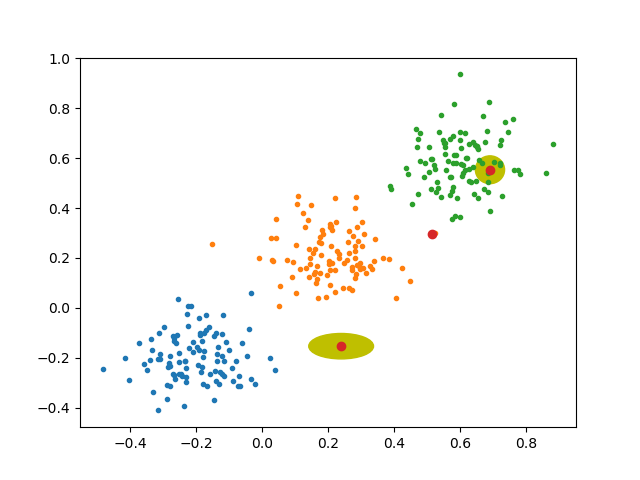
\includegraphics[width=7cm]{imgs/100_learn.png}}
% \subfigure[Epoch  B]{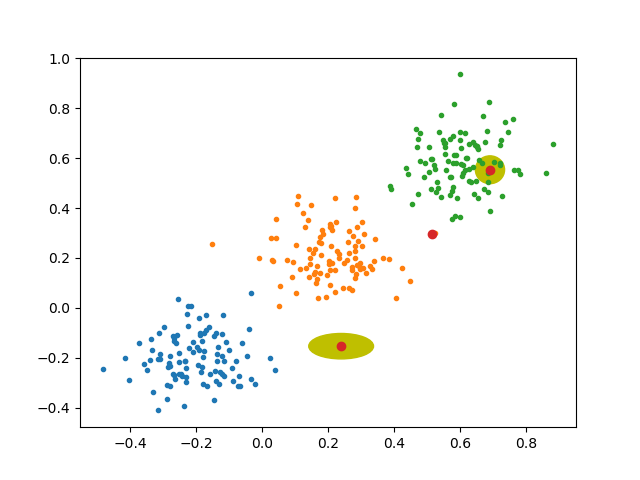
\includegraphics[width=7cm]{imgs/100_learn.png}}
% \subfigure[Epoch  B]{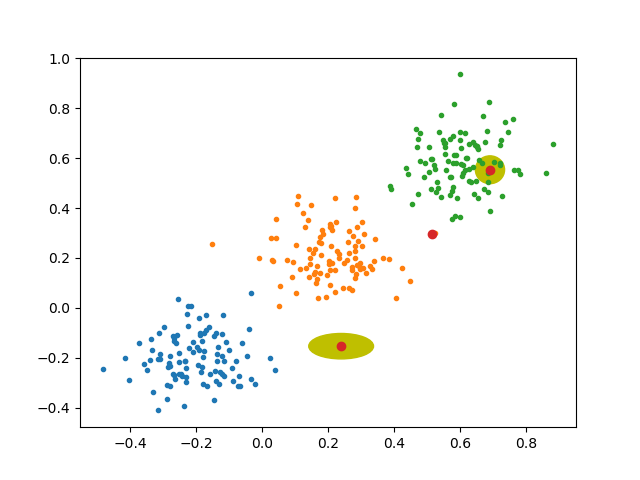
\includegraphics[width=7cm]{imgs/100_learn.png}}
% \caption{Title for both}
% \end{sidewaysfigure}

% \begin{sidewaysfigure}
% \subfigure[Epoch  A]{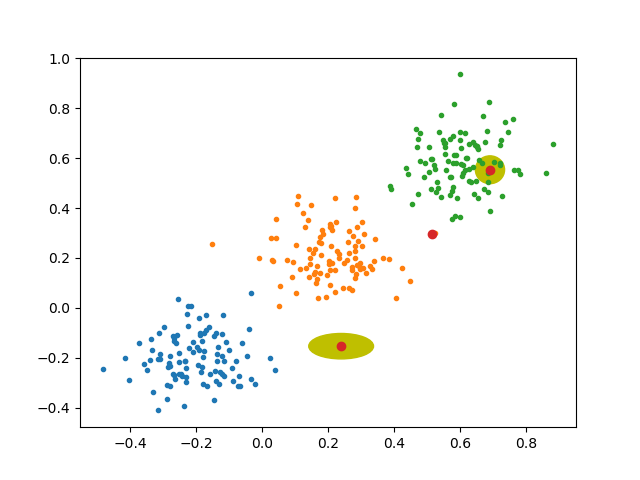
\includegraphics[width=7cm]{imgs/100_learn.png}}
% \subfigure[Epoch  B]{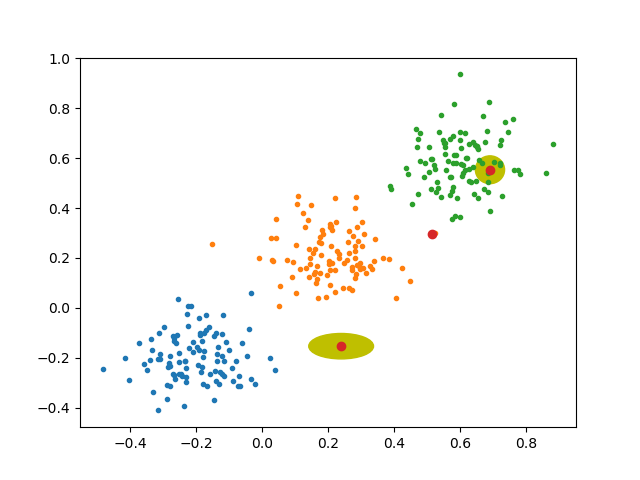
\includegraphics[width=7cm]{imgs/100_learn.png}}
% \subfigure[Epoch  B]{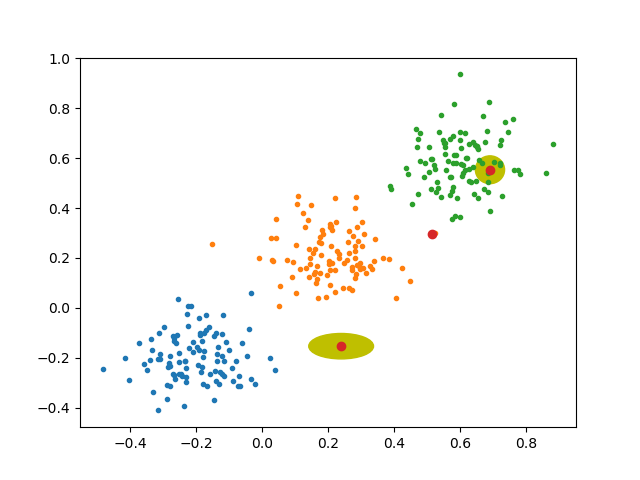
\includegraphics[width=7cm]{imgs/100_learn.png}}
% \caption{Title for both}
% \end{sidewaysfigure}

% \begin{sidewaysfigure}
% \subfigure[Epoch  A]{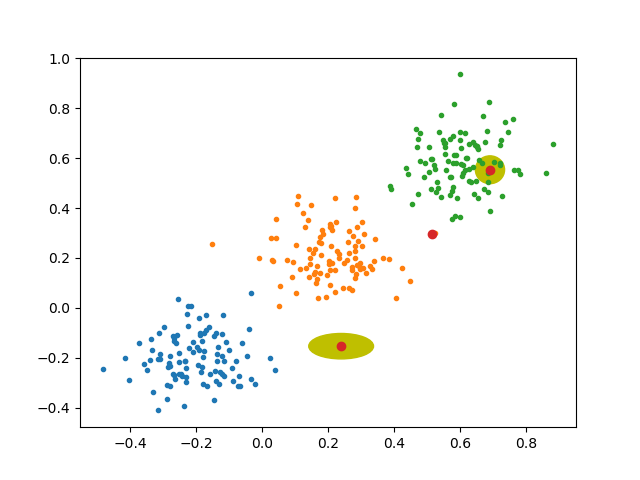
\includegraphics[width=7cm]{imgs/100_learn.png}}
% \subfigure[Epoch  B]{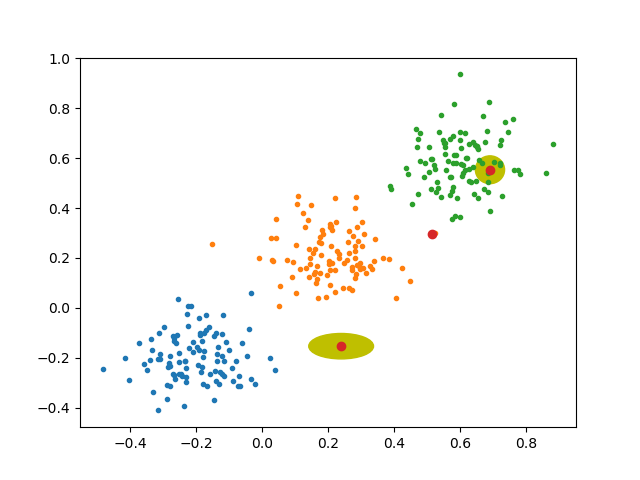
\includegraphics[width=7cm]{imgs/100_learn.png}}
% \subfigure[Epoch  B]{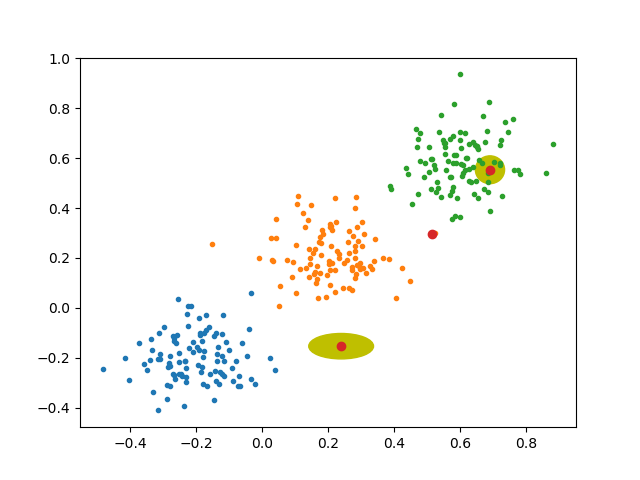
\includegraphics[width=7cm]{imgs/100_learn.png}}
% \caption{Title for both}
% \end{sidewaysfigure}




\section{Gaussian Mixture VAE}

\subsection{Detailed Description}

Here, fistly I introduce the the Gaussian Mixture VAE model (named GMVAE model). 
Based on the pre-designed model,  it uses $Discrete(\pi)$ as the prior for $Z$; and uses 
$N(\mu_{Z^{i}}, diag{\sigma_{Z^{i}}^{2}})$ as the prior for $H$, and then a feed-forword
neural network is used to learn the lantent representation with the input of $H$, finally 
$X$ is generated by a Bernoulli distribution which represent the 10 different type of digit 
image in the MNIST dataset.
\\
One method to solve this problem is  sum over $Z$ in the joint likelihood to get a joint likelihood
with only $H$ and $X$. In this model , the variational posterior distribution is 
\begin{equation}
    \begin{aligned}
        p(X,H)&= \sum_Z p(\textbf{X},\textbf{H},Z) \\
              &= p(X|H) \sum p(H|Z)p(Z) \\
        \log p(X,H) &= \log [p(X|H) \sum p(H|Z)p(Z)] \\
                    &= \log p(X|H) + \log \sum p(H|Z)p(Z) \\ 
        p(H, Z_i) &= p(H|Z_i)p(Z_i) \\
        p(H) &= \sum_{i=1}^K p(H,Z_i) \\
        p(X,H)  &= P(X|H)P(H) \\
        \log p(X,H) &= \log p(X|H) + \log p(H)
    \end{aligned}
\end{equation} 

$z$ is given by manully with the full range.
 $q(z|x)$ is Gaussian distribution, and the variational parameter $h$ is a Gaussian distribution, it would be the mean ($\mu$) and the variance ($\sigma$) of the latent variables for each image $\lambda_{x_i} = (\mu_{x_i}, \sigma^2_{x_i})$, 
Here I design a feed forword neural network to learn the best $\lambda$, the network consist of two layer fully connected.

\subsection{Data set}
The famous MNIST dataset is a large database of handwritten digits that is commonly used for training various image processing systems. The MNIST database contains 60,000 training images and 10,000 testing images.

\begin{figure}[!htbp]
\begin{center}

\includegraphics[width=10cm]{imgs/MNIST.png}
\end{center}
\caption{The MNIST dataset.}\label{datavis}
\end{figure}


\subsection{Experiment Setting}

\begin{enumerate}
\item[(1)] AdamOptimizer with Learning rate: 0.001.
\item[(2)] Using $zs.sgvb$ to estimate the gradient.
\item[(3)] Minimize the lower bound.

\end{enumerate}
Running on Tensorflow 1.1.0, K80-GPU, Ubuntu 14.04.

\subsection{Results}
The low bound curve shows that the training is convergent in 100 epoch. The low bound finally near to -0.83.

\begin{figure}[!htbp]
\begin{center}
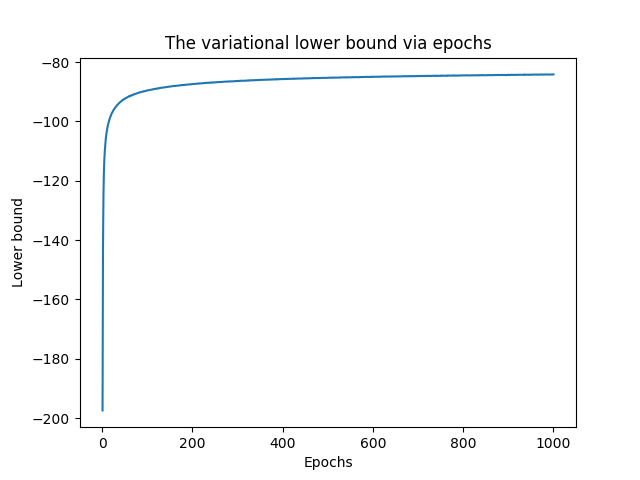
\includegraphics[width=12cm]{gmmvae2/lb.png}
\end{center}
\caption{The variational lower bound and surrogate cost via epochs.}\label{datavis}
\end{figure}

Next, I show the results of two experiment just run two times with the same parameter.
\\
\\
For experiment 1, we found that the model learn nothing in the first 10 epoch, and after 100 epoch, some $z$ specific digit image can be generate by a fixed $z$. For example, $z=9 and z=10$ (onehot vector) can generate images with 1, and $z = 8$ can generate images with zero, $z=3$ can generate images with six very good, but other $z$ are generating mixed type.


\begin{landscape}
\begin{figure}
\centering
\subfigure[Epoch 1]{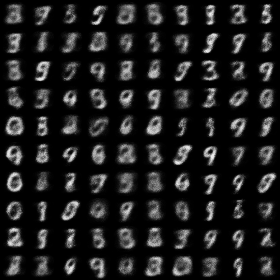
\includegraphics[width=6cm]{gmmvae/gmmvae.epoch.1.png}}
\subfigure[Epoch 10]{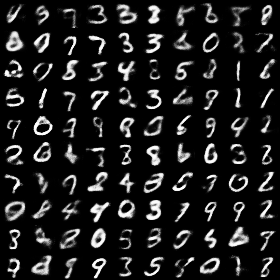
\includegraphics[width=6cm]{gmmvae/gmmvae.epoch.10.png}}
\subfigure[Epoch 100]{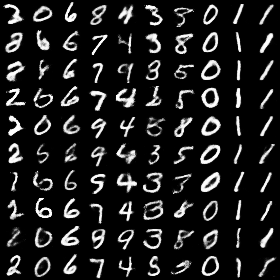
\includegraphics[width=6cm]{gmmvae/gmmvae.epoch.100.png}}
\vskip3ex
\subfigure[Epoch 200]{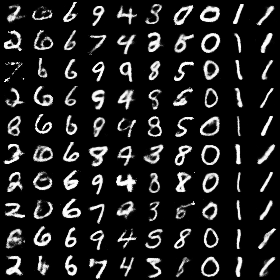
\includegraphics[width=6cm]{gmmvae/gmmvae.epoch.200.png}}
\subfigure[Epoch 300]{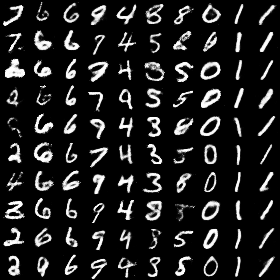
\includegraphics[width=6cm]{gmmvae/gmmvae.epoch.300.png}}
\subfigure[Epoch 400]{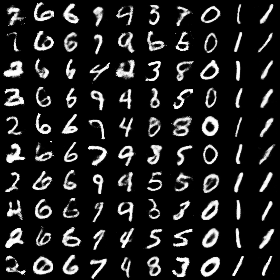
\includegraphics[width=6cm]{gmmvae/gmmvae.epoch.400.png}}

\caption{Experiment 1 for generating the image.}
\end{figure}
\end{landscape}

\begin{landscape}
\begin{figure}
\centering
\subfigure[Epoch 500]{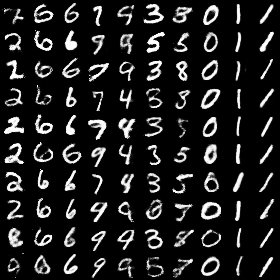
\includegraphics[width=6cm]{gmmvae/gmmvae.epoch.500.png}}
\subfigure[Epoch 600]{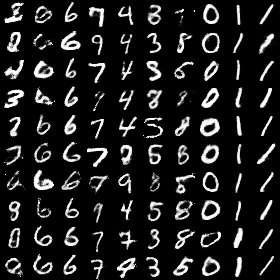
\includegraphics[width=6cm]{gmmvae/gmmvae.epoch.600.png}}
\subfigure[Epoch 700]{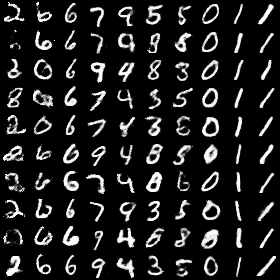
\includegraphics[width=6cm]{gmmvae/gmmvae.epoch.700.png}}
\vskip3ex
\subfigure[Epoch 800]{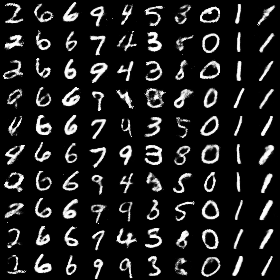
\includegraphics[width=6cm]{gmmvae/gmmvae.epoch.800.png}}
\subfigure[Epoch 900]{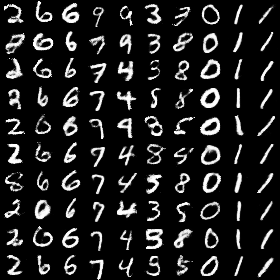
\includegraphics[width=6cm]{gmmvae/gmmvae.epoch.900.png}}
\subfigure[Epoch 1000]{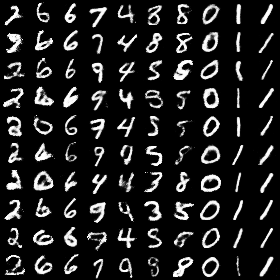
\includegraphics[width=6cm]{gmmvae/gmmvae.epoch.1000.png}}

\caption{Experiment 1 for generating the image.}
\end{figure}
\end{landscape}



\begin{landscape}
\begin{figure}
\centering
\subfigure[Epoch 1]{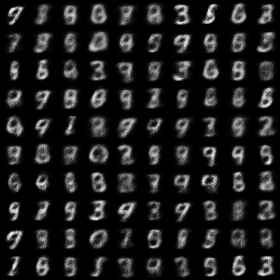
\includegraphics[width=6cm]{gmmvae2/gmmvae.epoch.1.png}}
\subfigure[Epoch 10]{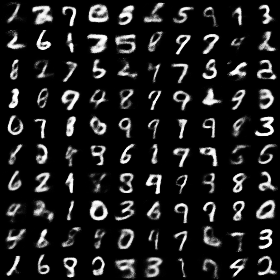
\includegraphics[width=6cm]{gmmvae2/gmmvae.epoch.10.png}}
\subfigure[Epoch 100]{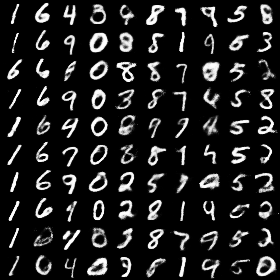
\includegraphics[width=6cm]{gmmvae2/gmmvae.epoch.100.png}}
\vskip3ex
\subfigure[Epoch 200]{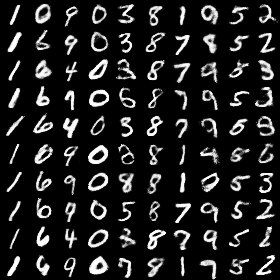
\includegraphics[width=6cm]{gmmvae2/gmmvae.epoch.200.png}}
\subfigure[Epoch 300]{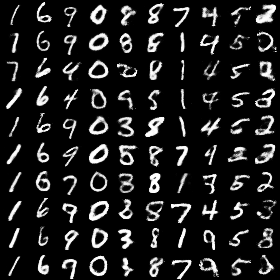
\includegraphics[width=6cm]{gmmvae2/gmmvae.epoch.300.png}}
\subfigure[Epoch 400]{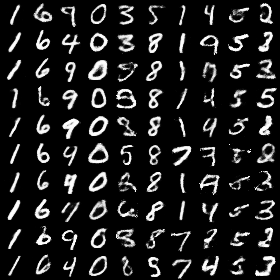
\includegraphics[width=6cm]{gmmvae2/gmmvae.epoch.400.png}}

\caption{Experiment 2 for generating the image.}
\end{figure}
\end{landscape}

\begin{landscape}
\begin{figure}
\centering
\subfigure[Epoch 500]{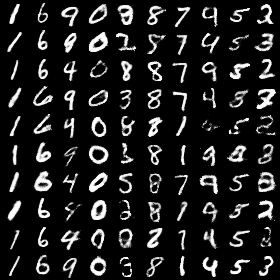
\includegraphics[width=6cm]{gmmvae2/gmmvae.epoch.500.png}}
\subfigure[Epoch 600]{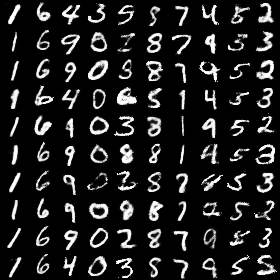
\includegraphics[width=6cm]{gmmvae2/gmmvae.epoch.600.png}}
\subfigure[Epoch 700]{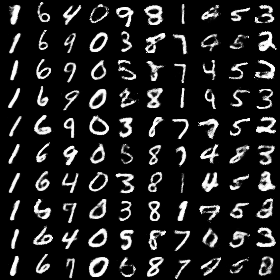
\includegraphics[width=6cm]{gmmvae2/gmmvae.epoch.700.png}}
\vskip3ex
\subfigure[Epoch 800]{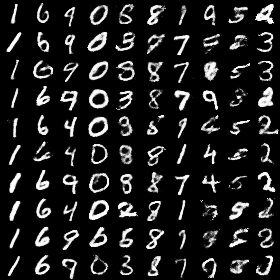
\includegraphics[width=6cm]{gmmvae2/gmmvae.epoch.800.png}}
\subfigure[Epoch 900]{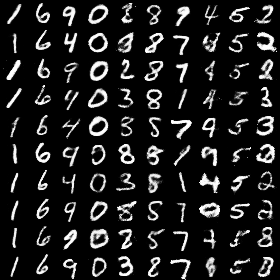
\includegraphics[width=6cm]{gmmvae2/gmmvae.epoch.900.png}}
\subfigure[Epoch 1000]{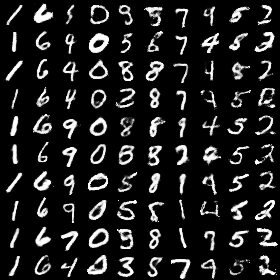
\includegraphics[width=6cm]{gmmvae2/gmmvae.epoch.1000.png}}

\caption{Experiment 2 for generating the image.}
\end{figure}
\end{landscape}


\section{Implemention}

 I implemented the algorithm using ZhuSuan. Code lists below.\\


%\begin{lstlisting}[language=Python]
Code of \textbf{vGM.py}\\
\begin{verbatim}
#!/usr/bin/env python
# -*- coding: utf-8 -*-

from __future__ import absolute_import
from __future__ import print_function
from __future__ import division
import os
import time

import tensorflow as tf
from tensorflow.contrib import layers
from six.moves import range
import numpy as np
import zhusuan as zs

from matplotlib.patches import Ellipse
import matplotlib as mpl
#%matplotlib inline
from matplotlib import pyplot as plt
mpl.use('Agg')

def sampleData(prng, nb_samples=100):
    """sample data.
    """
    x_coor=[]
    y_coor=[]
    t_train=[]
    #[2, 5.], [5., 2.],[7.,8.]
    classid=0
    for mu, sigma, marker in [(-.2, 0.1, 'o'), (0.2, 0.1, 's'), (0.6, 0.1, '+')]:
        x, y = prng.normal(loc=mu, scale=sigma, size=(2, nb_samples))
        x_coor.extend(x)
        y_coor.extend(y)
        t_train.extend([classid]*100)
        classid+=1
    x_train = np.column_stack([x_coor,y_coor])
    return x_train,t_train


resample=False
if resample:
    prng = np.random.RandomState(96917002)
    x_train, t_train=sampleData( prng)
    np.savez("data.npz",x_train, t_train)
    print("Sampling data")

r=np.load("data.npz")
x_train, t_train=r['arr_0'],r['arr_1']
x_train_cp = r['arr_0']
n_x = x_train.shape[1]

tf.set_random_seed(1237)
# Define model parameters
n_z = 3
K = 3
D = n_x

@zs.reuse('model')
def gmm(observed, n, K,D): #vae(observed, n, n_x, n_z):
    with zs.BayesianNet(observed=observed) as model:
        # Discrete GMM
        #Step.1: z ~ Discrete(pi)
        pi = tf.get_variable(name="pi",shape=[1,K],initializer=tf.constant_initializer
                                 (np.random.dirichlet(np.ones(K),size=1)),\
                        dtype=tf.float32)
        pi_n = tf.tile(pi,[n,1])
        z = zs.OnehotDiscrete('z', tf.log(pi_n),dtype=tf.float32)
        print("pi_shape:",pi.shape)
        print(z.sample(4).shape)
        miu = tf.get_variable(name="miu", initializer=tf.random_uniform_initializer(\
                minval=-0.3,maxval=0.7,dtype=tf.float32), shape=[K,D], dtype=tf.float32)
        sigma = tf.get_variable(name="sigma", initializer=tf.random_uniform_initializer(\
                minval=0,maxval=0.2,dtype=tf.float32), shape=[K,D], dtype=tf.float32)
        
        #miu_z = tf.matmul(tf.cast(z, dtype=tf.float32),miu)
        mean_x = tf.tensordot(tf.cast(z, dtype=tf.float32),miu, axes=1)
        print("mean_x:",tf.shape(mean_x))
        #sigma_z = tf.matmul(tf.cast(z, dtype=tf.float32),sigma)
        std_x = tf.tensordot(tf.cast(z, dtype=tf.float32),sigma, axes=1)
        print("std_x:",tf.shape(std_x))
        
        x = zs.Normal('x', mean_x, tf.log(std_x), group_event_ndims=1)
        print("x:",tf.shape(x))

    return model, x, miu, sigma, pi

# z inference
@zs.reuse('variational')
def q_net(x, n, K): #def q_net(x, n_z):
    with zs.BayesianNet() as variational:
        # Discrete GMM
        lz_x = layers.fully_connected(tf.to_float(x), 500)
        lz_x = layers.fully_connected(lz_x, 500)
        log_pi = layers.fully_connected(lz_x, K, activation_fn=None)
        z = zs.OnehotCategorical('z', log_pi,n_samples=n,  group_event_ndims=0,dtype=tf.float32)

    return variational,tf.arg_max(log_pi,dimension=1)

x = tf.placeholder(tf.float32, shape=[None, n_x], name='x')
n = tf.shape(x)[0]

def log_joint(observed):
    model, _ ,_ ,_,_ = gmm(observed, n, K, D)
    log_pz, log_px_z = model.local_log_prob(['z', 'x'])
    print("log_pz:", log_pz.shape)
    print("log_px_z:", log_px_z.shape)
    return tf.cast(log_pz + log_px_z, dtype=tf.float32)

variational,max_pi = q_net(x, n, K)
qz_samples, log_qz = variational.query('z', outputs=True,
                                           local_log_prob=True)

#Ocost, Olower_bound = zs.nvil(log_joint,\
#Ocost, Olower_bound = zs.nvil(log_joint,decay=tf.cast(0.2,dtype=tf.float32), variance_normalization=True,\
#Ocost, Olower_bound = zs.nvil(log_joint,decay=tf.cast(0.2,dtype=tf.float32),\
# === Amazing code
Ocost, Olower_bound = \
  zs.nvil(log_joint,\
    decay=tf.cast(0.2,dtype=tf.float32), \
    variance_normalization=True, \
    observed={'x': x}, \
  latent={'z': [tf.cast(qz_samples, dtype=tf.float32), tf.cast(log_qz, dtype=tf.float32)]})

Mcost = Ocost
Mlower_bound = tf.reduce_mean(Olower_bound)
optimizer = tf.train.AdamOptimizer(0.0001)
infer = optimizer.minimize(Mcost)

# Generate data
n_gen = 80
_, _, mean_x,std_x, pi  = gmm({}, n_gen, K, D)

# Define training parameters
epoches = 3000
batch_size = 80
iters = x_train.shape[0] // batch_size
save_freq = 200

def plotResult(iepoch):
    fig, ax = plt.subplots()
    
    
    ax.plot(x_train[0:100,0],x_train[0:100,1],".")
    ax.plot(x_train[101:200,0],x_train[101:200,1],".")
    ax.plot(x_train[201:,0],x_train[201:,1],".")
    
    x_means = sess.run(mean_x)
    print("x_means:",x_means)
    x_std = sess.run(std_x)
    print("x_std:",x_std)
    x_pi = sess.run(pi)
    
    #x_means= np.matmul(x_means,x_pi)
    ax.plot(x_means[:,0],x_means[:,1],'o')
    
    #mean = [ 19.92977907 ,  5.07380955]
    widths = 3*(x_std[:,0])
    heights = 3*(x_std[:,1])
    angle = 0
    ells = [mpl.patches.Ellipse(xy=x_mean, width=width, height=height, \
            angle = angle, color="y") for i, (x_mean, width, height) in \
            enumerate(zip(x_means, widths, heights))]
    

    [ax.add_patch(ell) for ell in ells ]
    fig.savefig('./gmm/'+str(iepoch)+'_learn.png')
    #fig.tight_layout()
    #plt.show()

with tf.Session() as sess:
    sess.run(tf.global_variables_initializer())
    lbes= []
    costses = []
    for epoch in range(1, epoches + 1):
        np.random.shuffle(x_train_cp)
        lbs = []
        costs = []
        pis = []
        for t in range(iters):
            x_batch = x_train_cp[t * batch_size:(t + 1) * batch_size]
            _, lb, cost,x_mean, tmp_pi = sess.run([infer,Mlower_bound, Mcost, mean_x, pi],
                             feed_dict={x: x_batch})
            lbs.append(lb)
            costs.append(cost)
            pis.extend(tmp_pi)
        m_pis = np.asarray(pis)
        print('Epoch {}: Lower bound = {}, Cost = {}, Pi = {}'.format(
            epoch, np.mean(lbs), np.mean(costs),np.mean(m_pis,axis=1)))
        lbes.append(np.mean(lbs))
        costses.append(np.mean(costs))
        if epoch % save_freq == 0:
            plotResult(epoch)
    fig_size = [16, 8]
    fig, axes = plt.subplots(ncols=2, nrows=1, num=0,
                             figsize=fig_size, squeeze=True)
    axes[0].plot(range(1, epoches + 1),lbes)
    axes[0].set_ylabel('Lower bound')
    axes[0].set_xlabel('Epochs')
    axes[0].set_title('The variational lower bound via epochs')
    axes[0].legend(loc='center right', shadow=True)
    axes[1].plot(range(1, epoches + 1),costses)
    axes[1].set_ylabel('Surrogate Cost')
    axes[1].set_xlabel('Epochs')
    axes[1].set_title('The Surrogate Cost bound via epochs')
    axes[1].legend(loc='upper right', shadow=True)
    fig.savefig('./gmm/cost_lb.png')

          

\end{verbatim}

Code of running \textbf{GMVAE.py}\\
\begin{verbatim}
#!/usr/bin/env python
# -*- coding: utf-8 -*-

from __future__ import absolute_import
from __future__ import print_function
from __future__ import division
import os

import tensorflow as tf
from tensorflow.contrib import layers
from six.moves import range
import numpy as np
import zhusuan as zs

from examples import conf
from examples.utils import dataset, save_image_collections
import warnings
warnings.filterwarnings("ignore")

tf.reset_default_graph()

@zs.reuse('model')
def gmmvae(observed, n_x, N, D, K):
    with zs.BayesianNet(observed=observed) as model:
        pi_ = tf.get_variable(name='pi',shape=[K], dtype = tf.float32, \
                              initializer = tf.random_uniform_initializer(minval=0.,\
                                maxval=0., dtype=tf.float32))
        # N*K
        pi_ = tf.tile(tf.expand_dims(pi_,0),[N,1]) 
        # N*K
        z = zs.OnehotDiscrete('z',pi_, dtype = tf.float32, group_event_ndims=0)
        # K*D
        h_mean = tf.get_variable(name='mean_h', dtype=tf.float32, shape=[K, D],\
                                  initializer=tf.random_uniform_initializer(minval=0.,\
                                    maxval=1,seed=None, dtype=tf.float32))
        # K*D
        h_sigma = tf.get_variable(name = 'sigma_h', dtype = tf.float32, shape=[K, D],\
                                  initializer=tf.random_uniform_initializer(minval=0.,\
                                    maxval=1, seed=None,dtype=tf.float32))
                                   #initializer = tf.random_uniform([K,D], dtype=tf.float32))
        # N*D
        h_mean = tf.matmul(z, h_mean)
        h_sigma = tf.matmul(z, h_sigma)
        # N*D
        h = zs.Normal('h', h_mean, h_sigma, group_event_ndims=1)
        fNN = layers.fully_connected(tf.to_float(h), 500)
        fNN = layers.fully_connected(fNN, 500)
        # N*n_x
        x_logits = layers.fully_connected(fNN, n_x, activation_fn=None)
        x = zs.Bernoulli('x', x_logits, group_event_ndims=1, dtype=tf.float32)
        return model, x_logits

@zs.reuse('variational')
def q_net(x, n_x, N, D, K):
    with zs.BayesianNet() as variational:
        # N*n_x
        fNN1 = layers.fully_connected(tf.to_float(x), 500)
        fNN1 = layers.fully_connected(fNN1, 500)
        h_mean = layers.fully_connected(fNN1, D, activation_fn=None)
        h_sigma = layers.fully_connected(fNN1, D, activation_fn=None)
        h = zs.Normal('h',h_mean,h_sigma,group_event_ndims=1)
        return variational

if __name__ == "__main__":
    # Load MNIST
    data_path = os.path.join(conf.data_dir, 'mnist.pkl.gz')
    x_train, t_train, x_valid, t_valid, x_test, t_test = \
    dataset.load_mnist_realval(data_path)
    x_train = np.random.binomial(1, x_train, size=x_train.shape)
    n_x = x_train.shape[1]  # 784,shape=(50000,784)
    D = 40
    K = 10
    batch_size = 256
    N = batch_size

    x = tf.placeholder(tf.float32, shape=[None, n_x], name='x')
    
    def sum_z_log_joint(observed,N,K):
        ober_z = np.eye(K)
        sum_z = []
        #sum_z = 0
        for i in range(K):
            ober_zi = np.tile(ober_z[i,], [N,1])
            observed['z'] = ober_zi 
            model, _ = gmmvae(observed, n_x, N, D, K)       # only need the model
            log_pz, log_ph_z = model.local_log_prob(['z','h'])
            sum_z.append(log_pz+ log_ph_z)
            #sum_z+= tf.exp(log_pz+ log_ph_z)
        return tf.reduce_logsumexp(sum_z, axis = 0)
        #return tf.log(sum_z)

    def log_joint(observed):
        log_ph = sum_z_log_joint(observed, N, K)
        model, _ = gmmvae(observed, n_x, N, D, K)        
        log_px_h = model.local_log_prob(['x'])
        return log_px_h  + log_ph

    variational = q_net(x, n_x, N, D, K)

    qh_samples, log_qh = variational.query('h', outputs=True,local_log_prob=True)
    qh_samples = tf.cast(qh_samples, dtype=tf.float32)
    log_qh = tf.cast(log_qh, dtype=tf.float32)

    lower_bound = tf.reduce_mean(
        zs.sgvb(log_joint,observed={'x': x},latent={'h':[qh_samples, log_qh]}))

    optimizer = tf.train.AdamOptimizer(0.001)
    infer = optimizer.minimize(-lower_bound)

    # Generate images
    n_gen = 100
    ober_z = np.eye(K)
    ober_z = np.tile(ober_z, [n_gen,1])

    _, x_logits= gmmvae({'z':ober_z}, n_x, n_gen, D, K)
    # only need the x_logits: N*D
    x_gen = tf.reshape(tf.sigmoid(x_logits), [-1, 28, 28, 1]) # N*28*28*1
    # Define training parameters
    epoches = 1000
    iters = x_train.shape[0] // batch_size  #50000/128=390
    save_freq = 1

    with tf.Session() as sess:
        sess.run(tf.global_variables_initializer())
        lbes= [] 
        for epoch in range(1, epoches + 1):
            np.random.shuffle(x_train)
            lbs = []
            for t in range(iters):
                x_batch = x_train[t * batch_size:(t + 1) * batch_size]
                _, lb = sess.run([infer, lower_bound], feed_dict={x: x_batch})
                lbs.append(lb)
            print('Epoch {}: Lower bound = {}'.format(epoch, np.mean(lbs)))
            lbes.append(np.mean(lbs))
            if epoch % save_freq == 0:
                images = sess.run(x_gen)  # gen batch-szie images
                name = "results/gmmvae/gmmvae.epoch.{}.png".format(epoch)
                save_image_collections(images, name)
        fig_size = [16, 8]
        fig, ax = plt.subplots()
        ax.plot(range(1, epoches + 1),lbes)
        ax.set_ylabel('Lower bound')
        ax.set_xlabel('Epochs')
        ax.set_title('The variational lower bound via epochs')
        ax.legend(loc='center right', shadow=True)
        
        fig.savefig('results/gmmvae/lb.png')

\end{verbatim}



\bibliographystyle{plain}
%\bibliography{bibliography.bib}
\end{document}